\documentclass[a4paper,10pt]{article}
\usepackage[utf8x]{inputenc}
\usepackage{placeins}
\usepackage{graphicx}
\usepackage{float}

%opening
\title{Draft}
\author{OJH}

\begin{document}

\maketitle

\begin{abstract}

\end{abstract}

\section{Results}
Throughout this results section, we present model data for the vertical velocity, $w$,  and
potential temperature, $b$ fields, since both are influential in the organisation convection. Any
region with positive $w$, and high $b$ is likely to trigger convection, with the opposite likely to
suppress triggering.

\subsection{The Effect of Raising the Position of the Rigid Lid Upper Bound-
ary Condition}
Figure  depicts the effect of increasing the
altitude of the upper lid. We observe the distribution of energy increases aloft, indicating a
radiative effect. Quantitative insights into the upward flux of energy may be obtained from this
data. For example, it appears that as the lid height increases the vertical flow at the top of plot
windows becomes more uniform.

\begin{figure}
  \caption{}
  \centering
    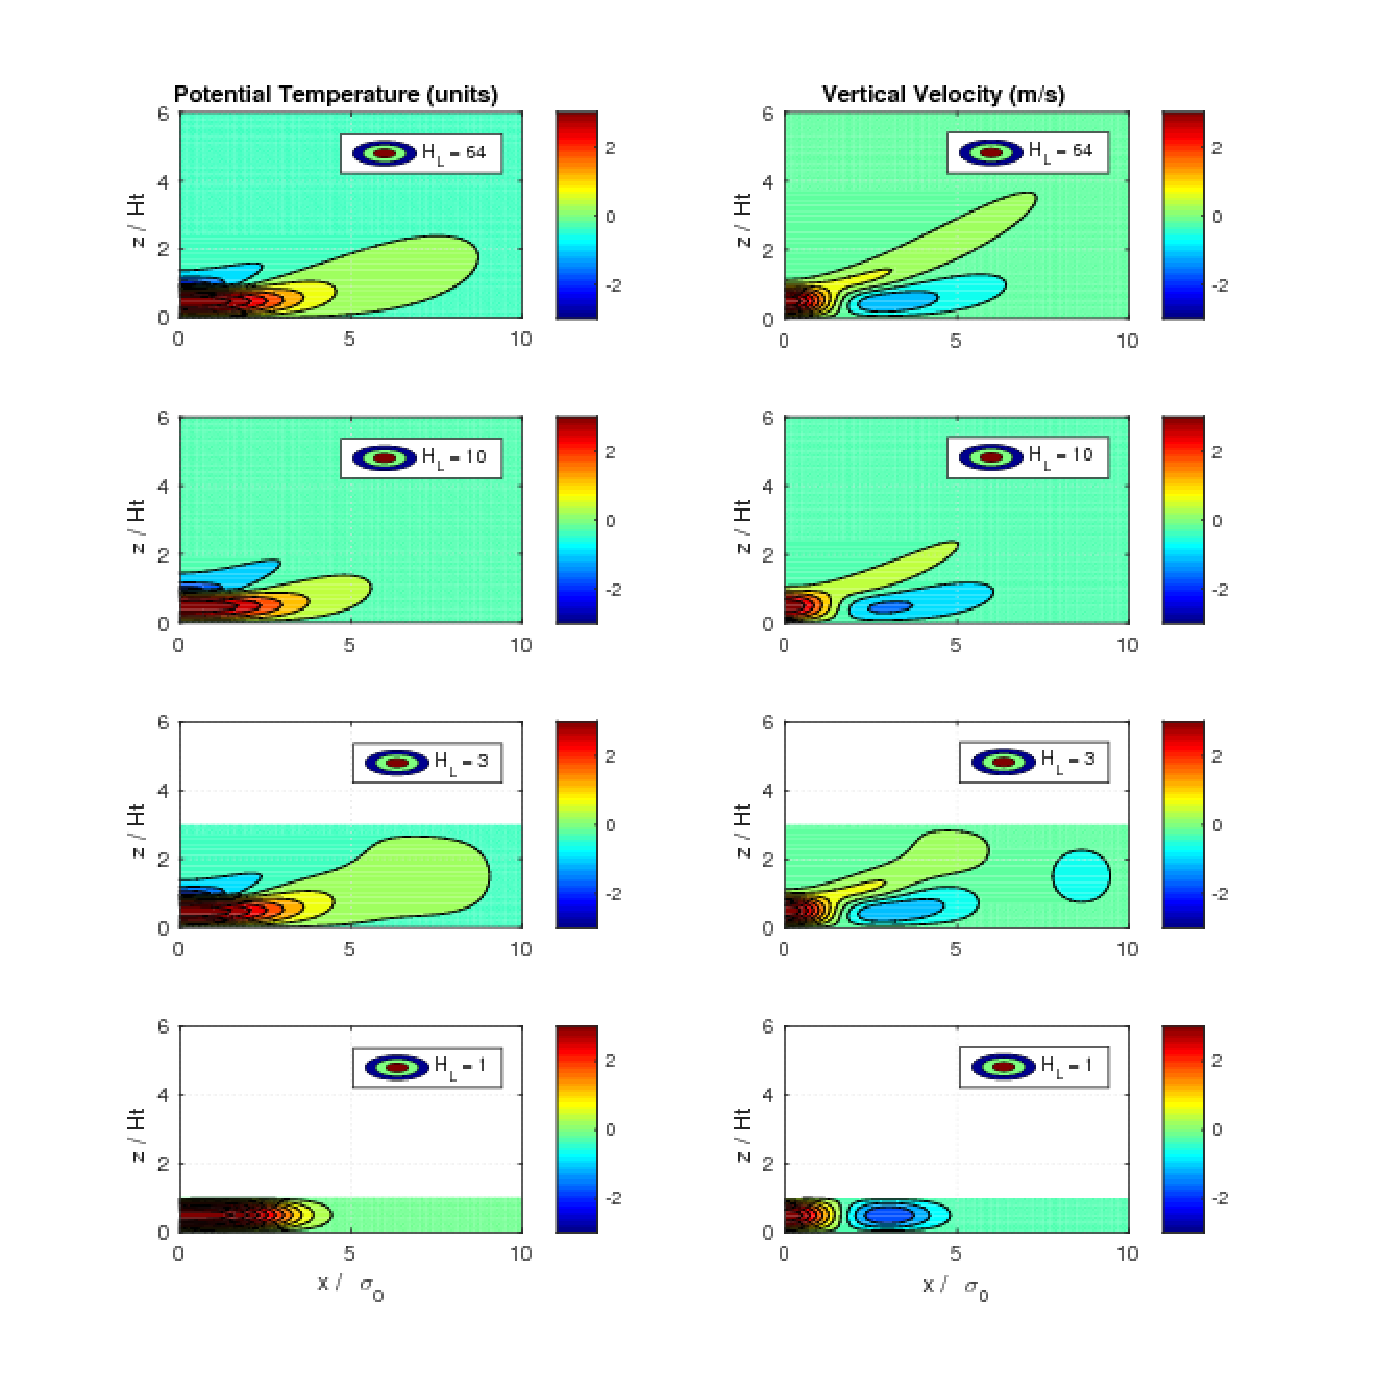
\includegraphics[width=1\textwidth]{raise_lid_t1.pdf}
  \label{raise_lid_t1}
\end{figure}

\begin{figure}
  \caption{}
  \centering
    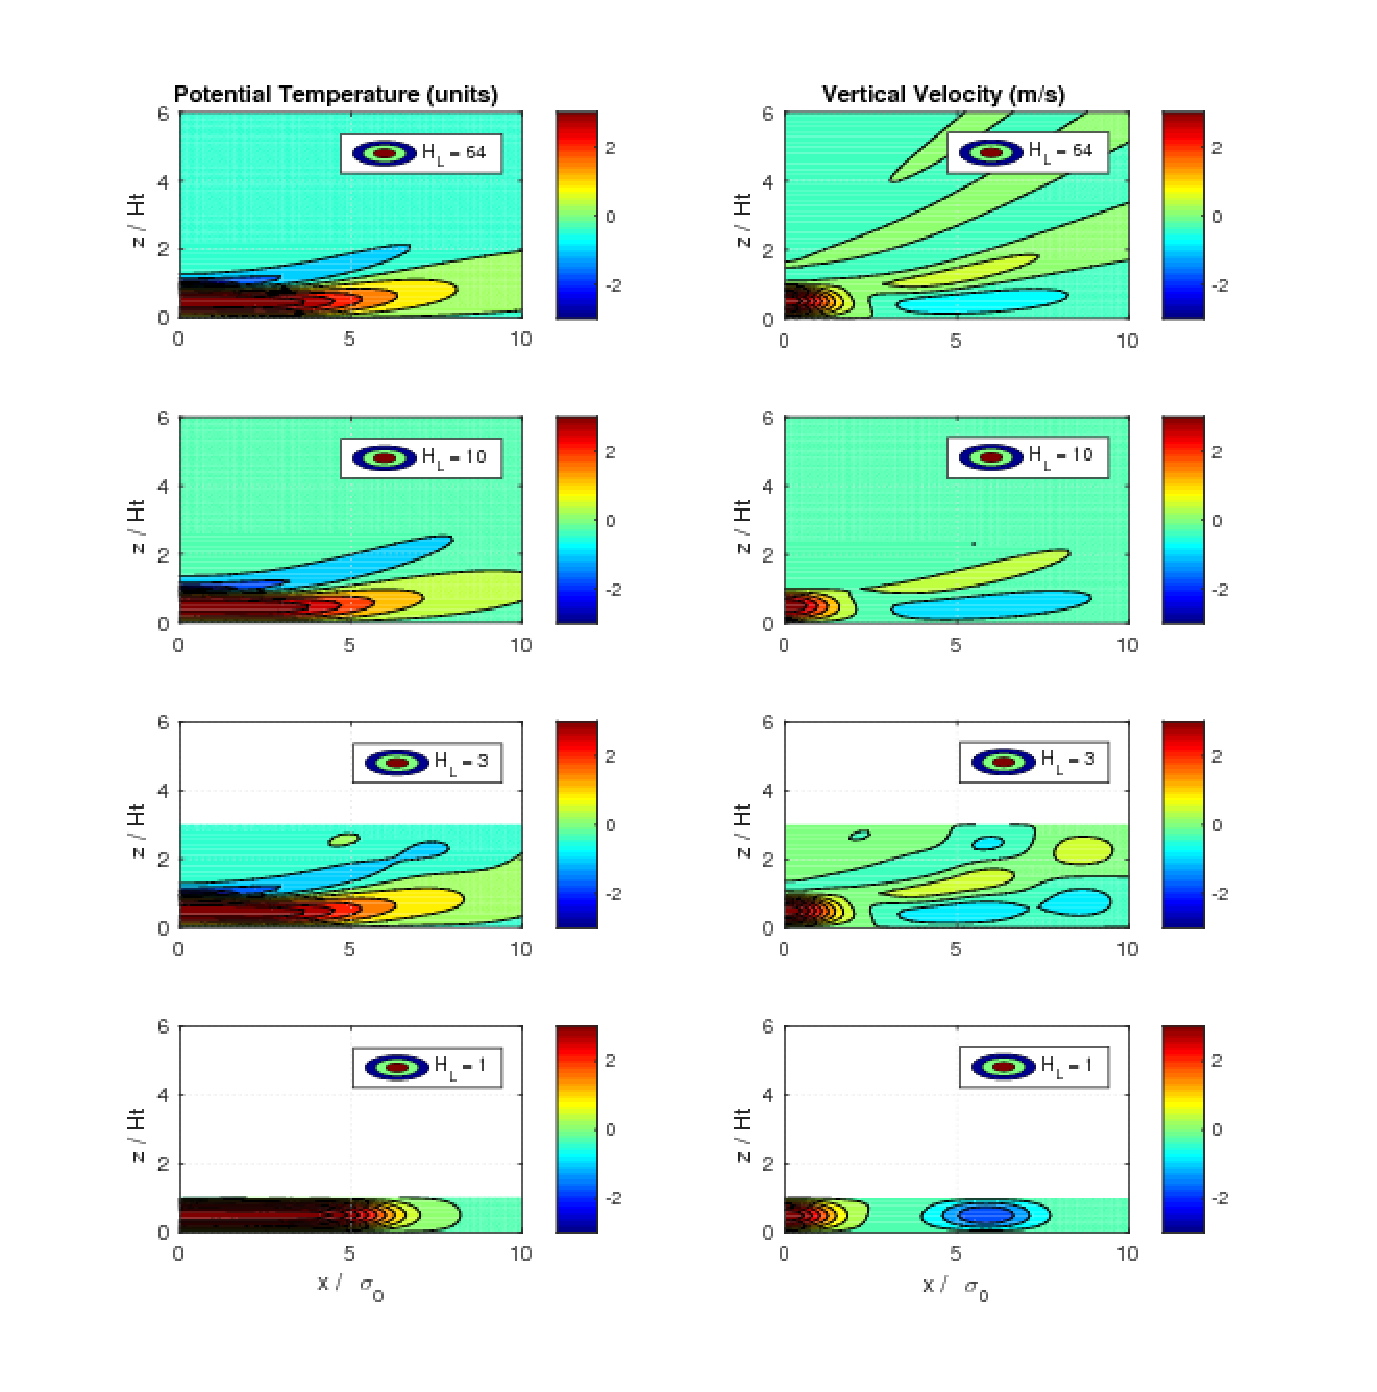
\includegraphics[width=1\textwidth]{raise_lid_t2.pdf}
  \label{raise_lid_t2}
\end{figure}

%\Floatbarrier

Along with figure  we note the horizontal evolution of the w-response, which
is characterised by modes with phase speed $\frac{N H}{j \pi}$ (recall $j$ is the vertical
harmonic number) is qualitatively unaffected by the process of raising the lid. The vertical
structure however varies considerably more between $H_L = 1$ and  $H_L = 3$ than it does between
$H_L = 10$ and $H_L = 64$ which is indicative of convergence of the $w$ and $b$ solution (at least
in the troposphere). We also note that as the height of the lid increases the influences of
the heating excite a deeper mode, characterised by a larger horizontal phase speed, as
expected. The confining effect of the lid intensifies subsidence in the troposphere, meaning
neighbouring convection is unlikely to be triggered. However, continuity considerations suggest
enhanced triggered elsewhere. In the present case, we
observe the only candidate region for this amplified ascent would be the heated region. We note that
the horizontal suppression of convection is more locally intense, but less mobile, in the trapped
cases.

One can better understand the time evolution of the system through figure HERE
%(\ref{Hovmoller_steady.eps})

\subsection{Transient Heating}
Assigning the time dependence of the heating function to be a simple boxcar function (on/off), we
investigate the influence of a transient heat source. Figure
 shows the $w$ and $b$ response
field to such transient heating which is switched off at a time $t = 30mins$ (a reasonably
realistic convection timescale, note). Advancing down the panels, we evolve at a time step of 15
minutes.

\begin{figure}
  \caption{}
  \centering
    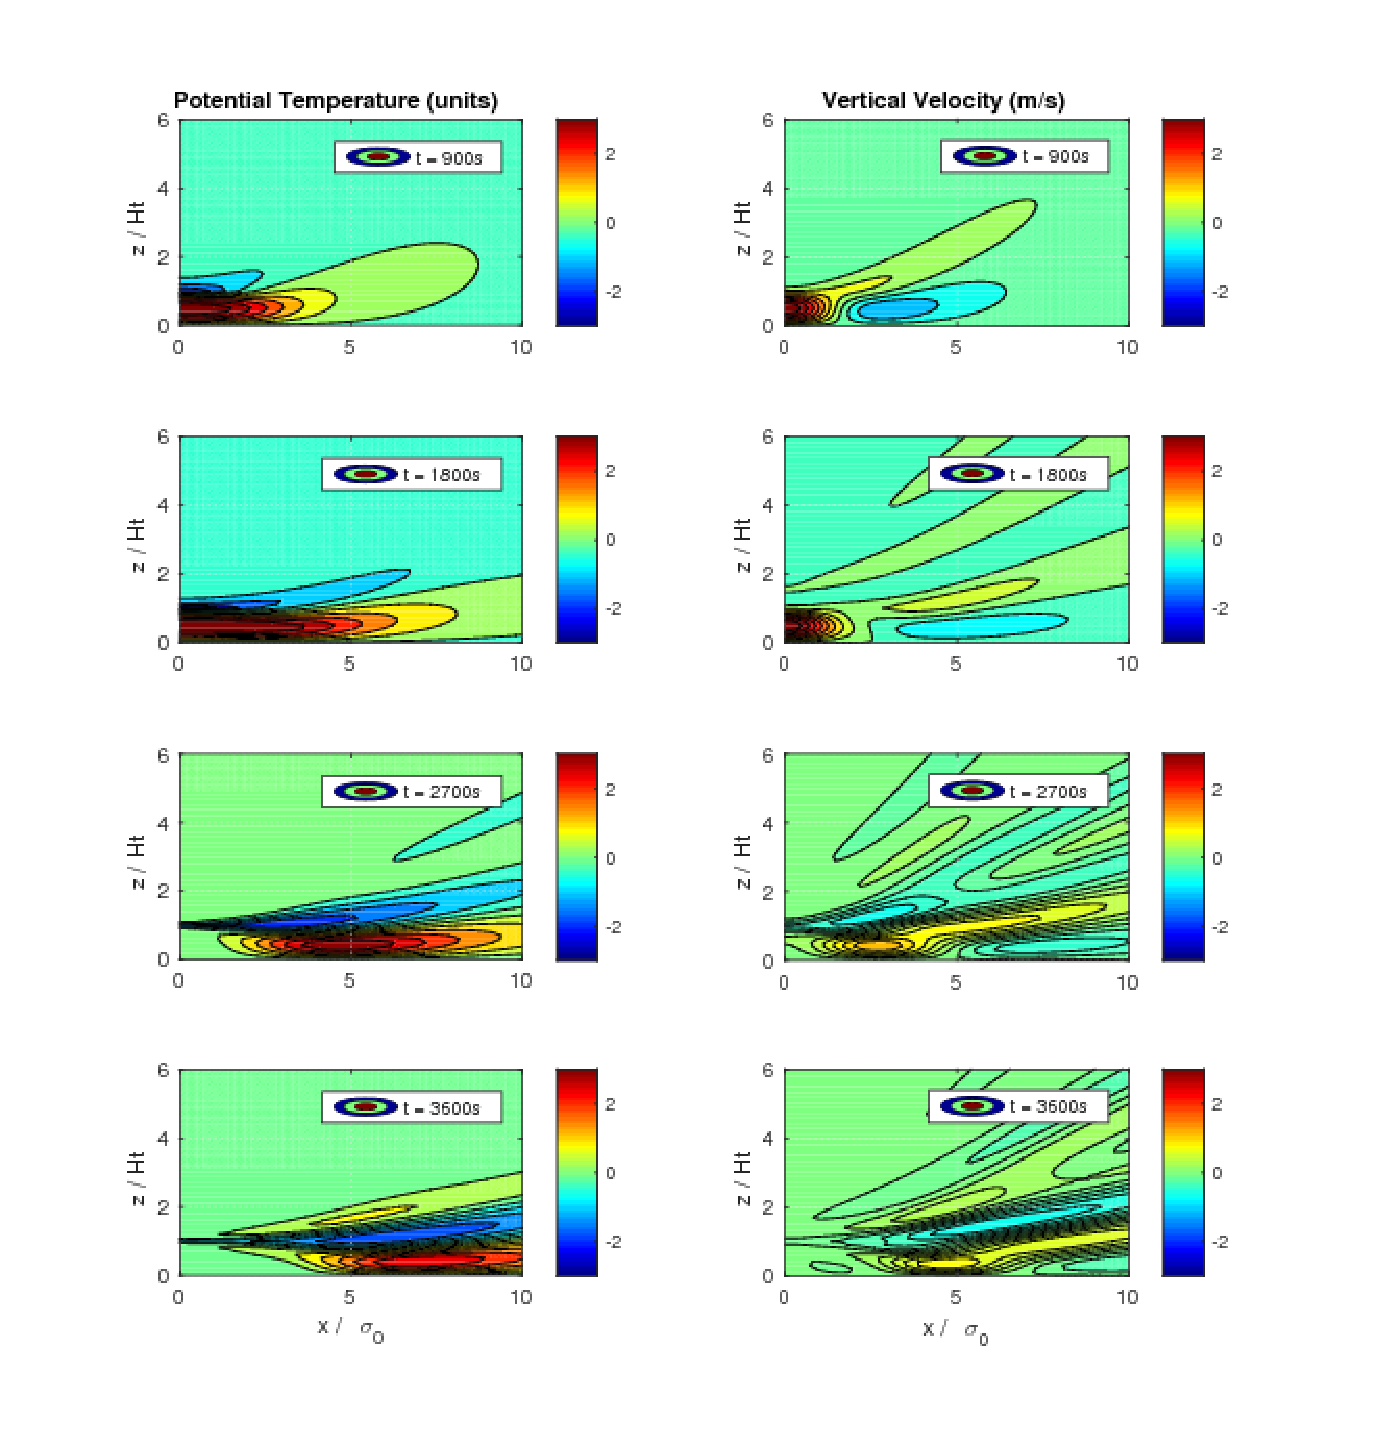
\includegraphics[width=1\textwidth]{Transient_vertical_cross.pdf}
  \label{vertical_cross_transient}
\end{figure}

%\Floatbarrier

The most notable effect of truncating heating is the occurrence a propagating region of ascent in
the troposphere (as seen in figure ), which is absent in all
the steady heating cases considered previously. 
% \begin{figure}
%   \caption{}
%   \centering
%     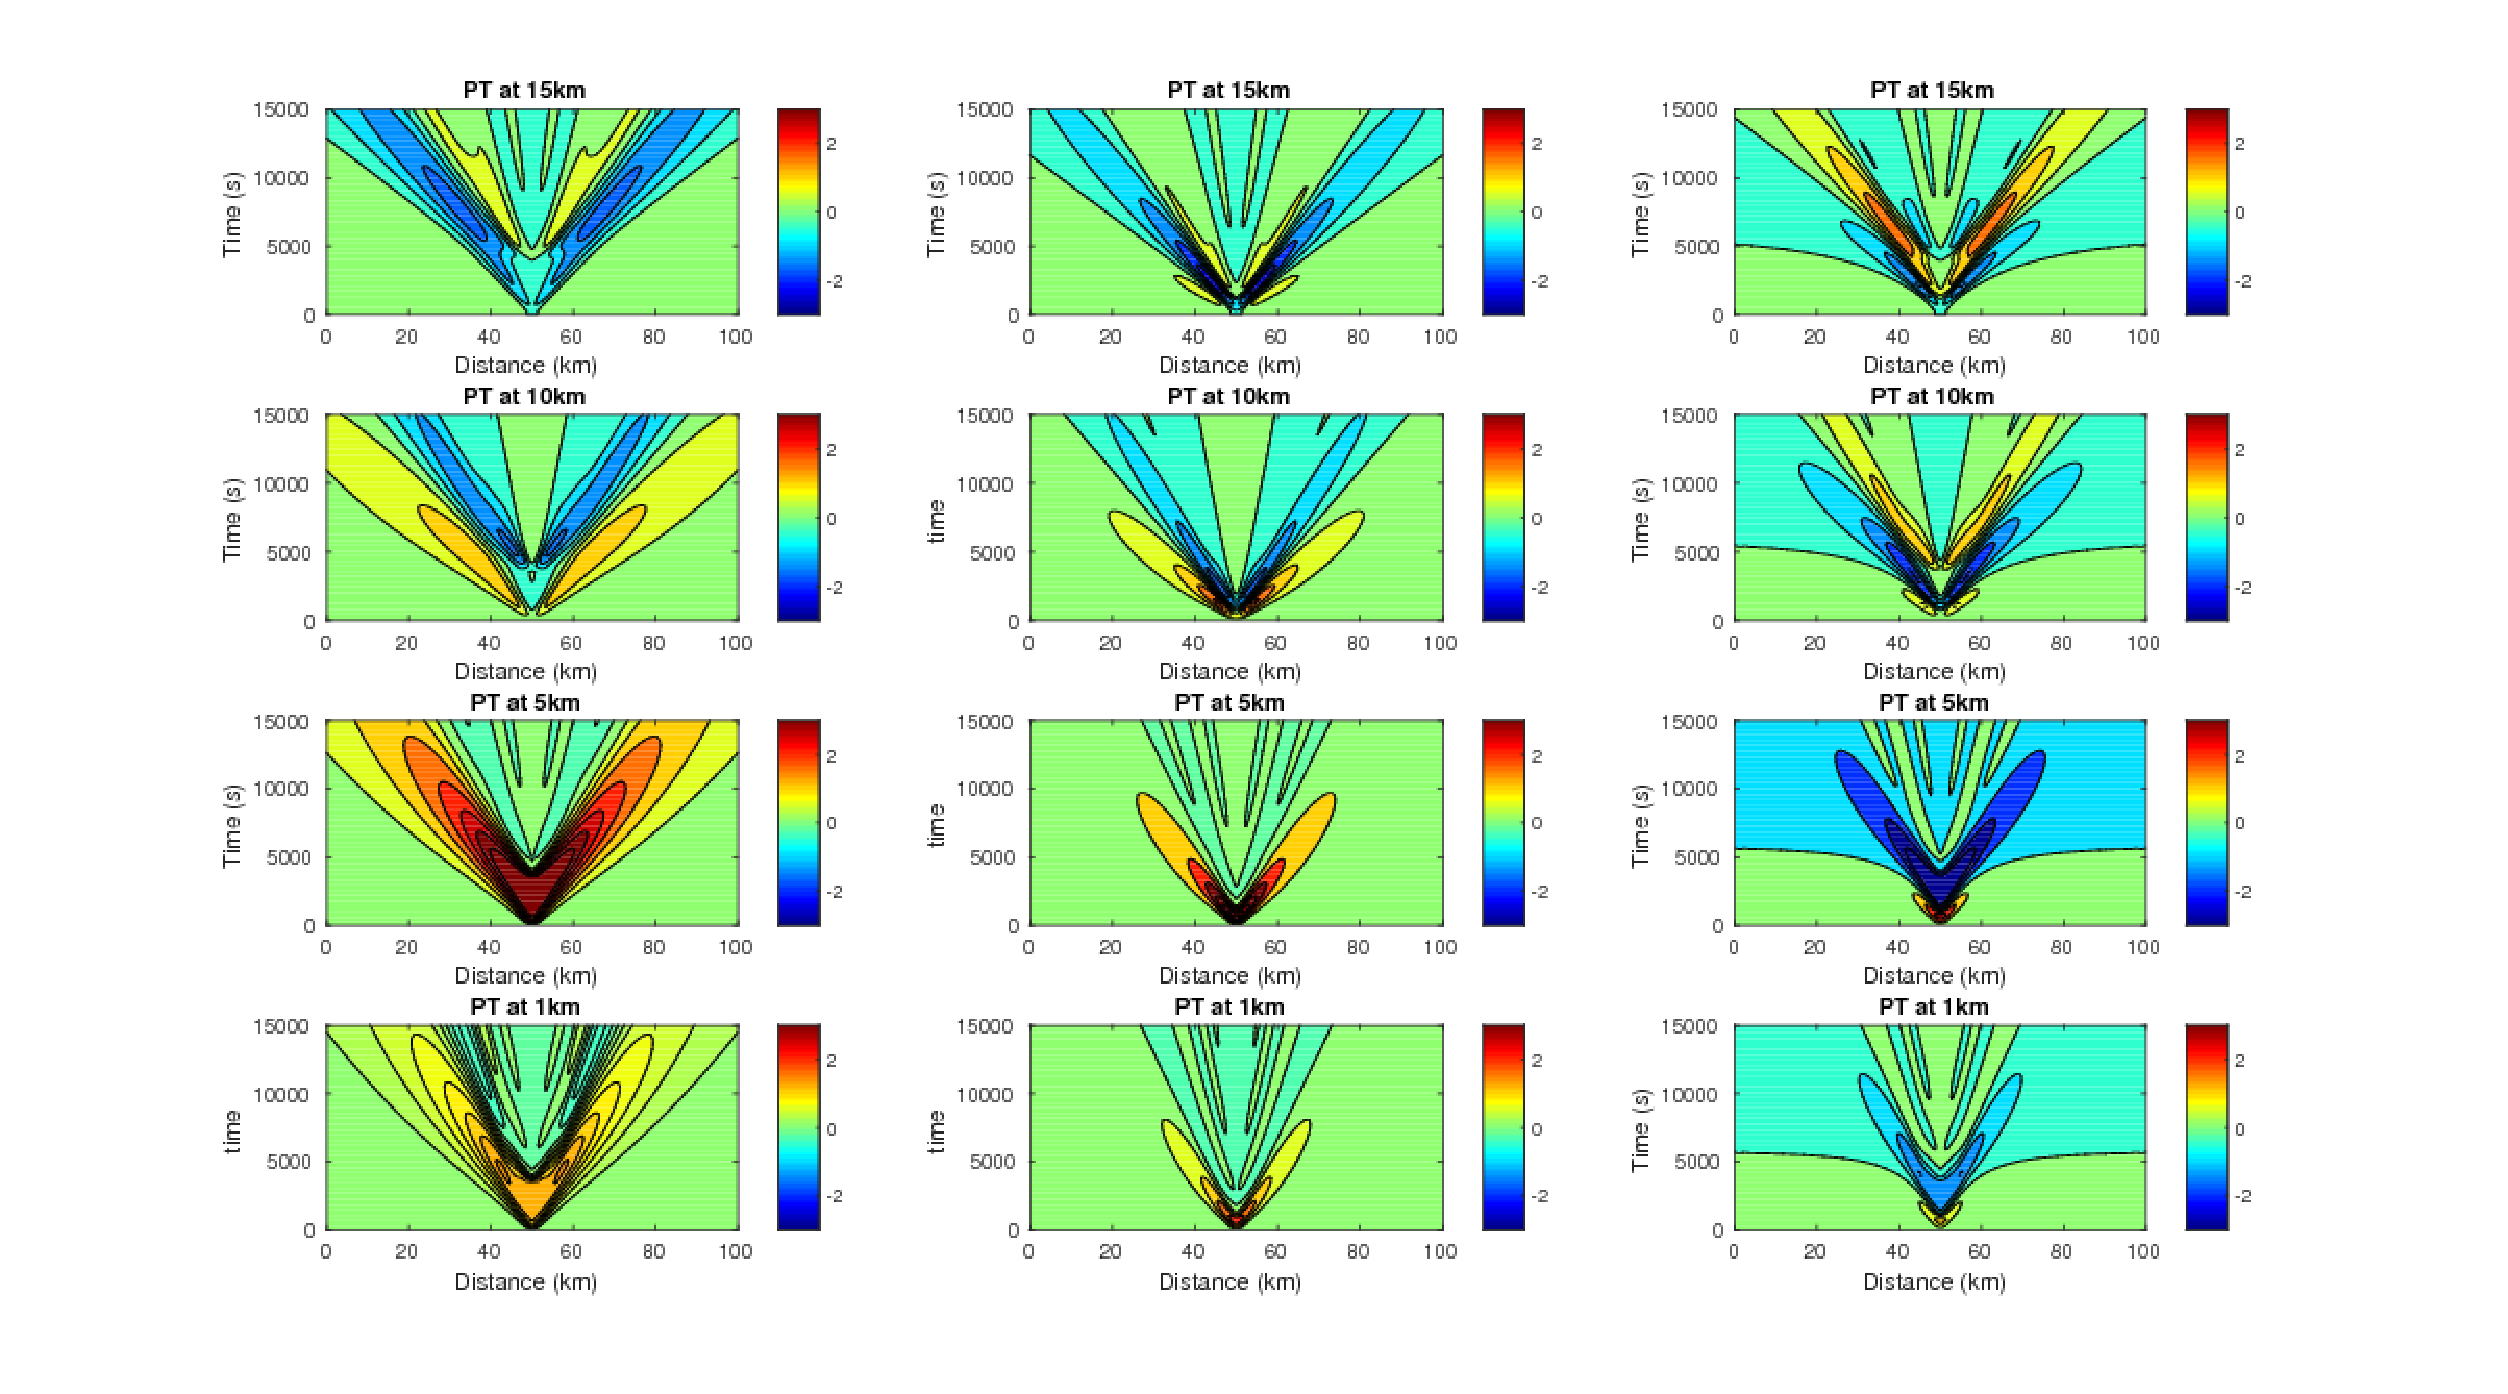
\includegraphics[width=1\textwidth]{hovmoller_transient_diffs.jpg}
%   \label{Hovmoller_transient_diffs}
% \end{figure}

%\Floatbarrier


HERE The reader is directed to the top right hand panel of
figure , in the region of $x = 2$. Counterintuitively, this observation appears to suggest that
terminating heating could trigger a weak convective event in the neighbourhood.


\subsection{TO INCLUDE}
\begin{figure}
  \caption{}
  \centering
    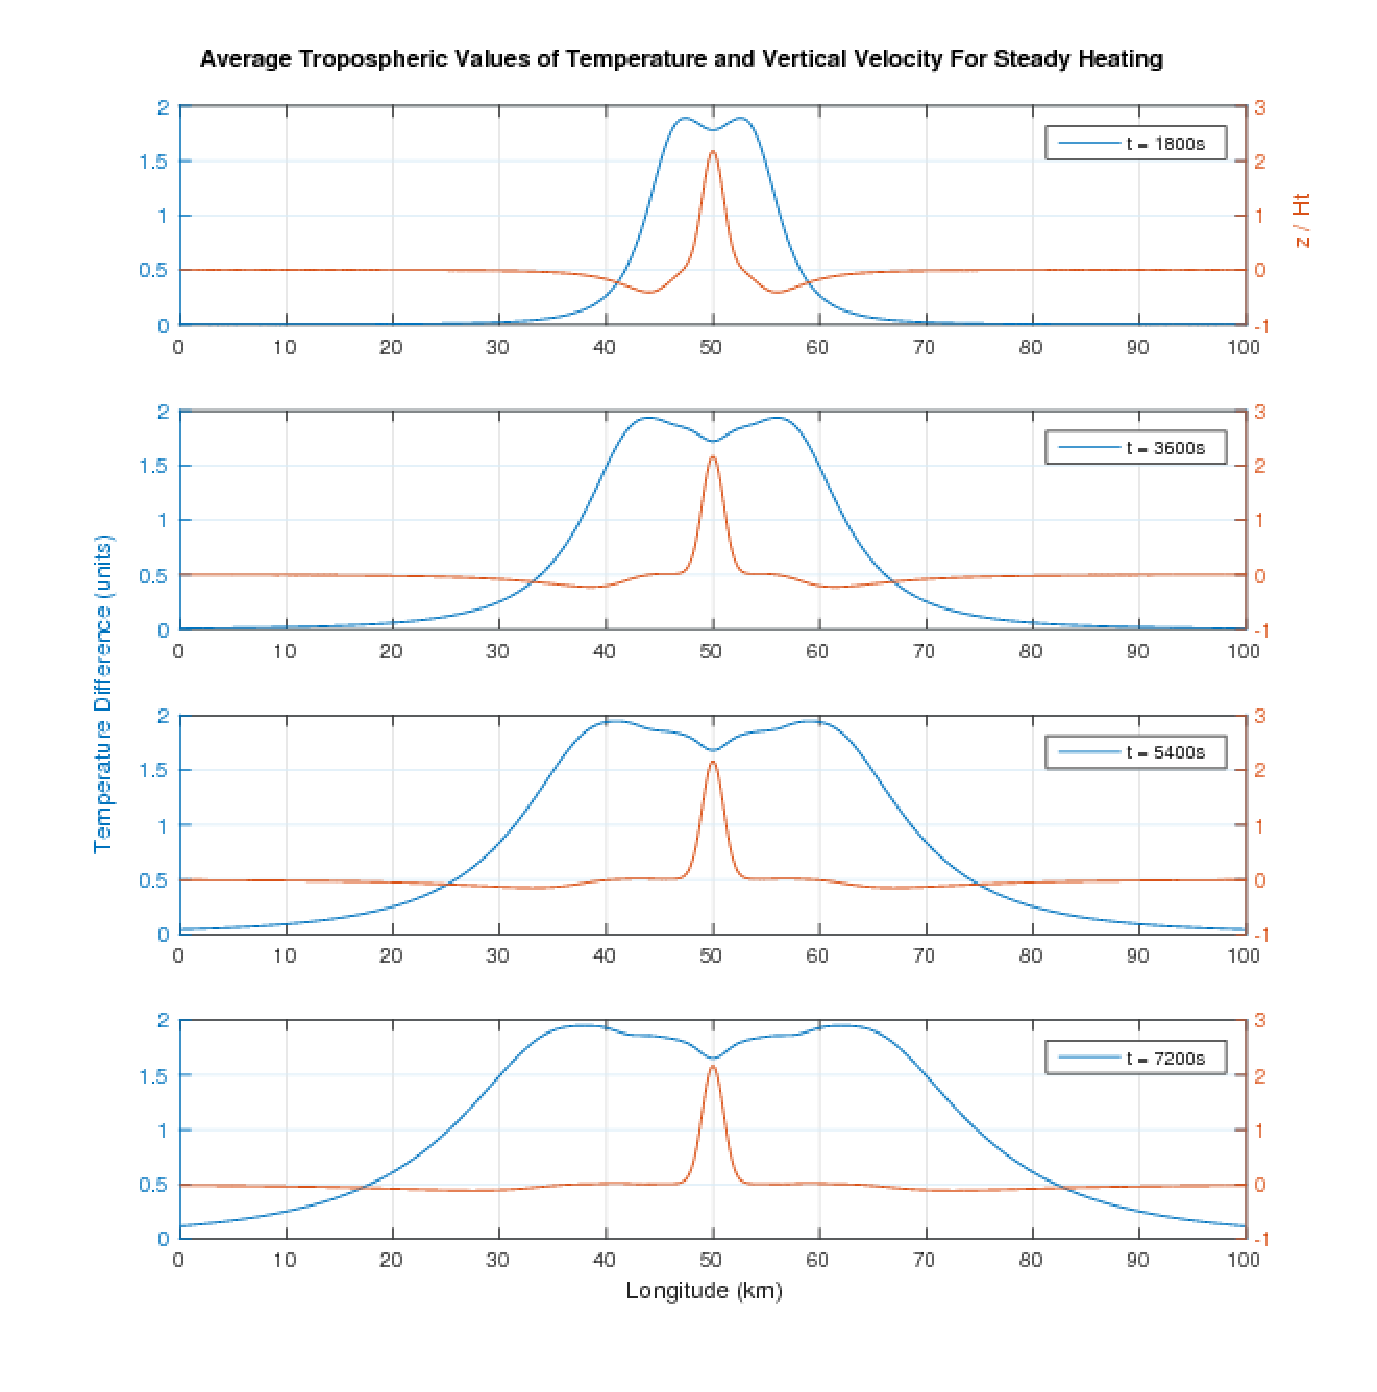
\includegraphics[width=1\textwidth]{trop_values_steady.pdf}
  \label{trop_values_steady}
\end{figure}

\begin{figure}
  \caption{}
  \centering
    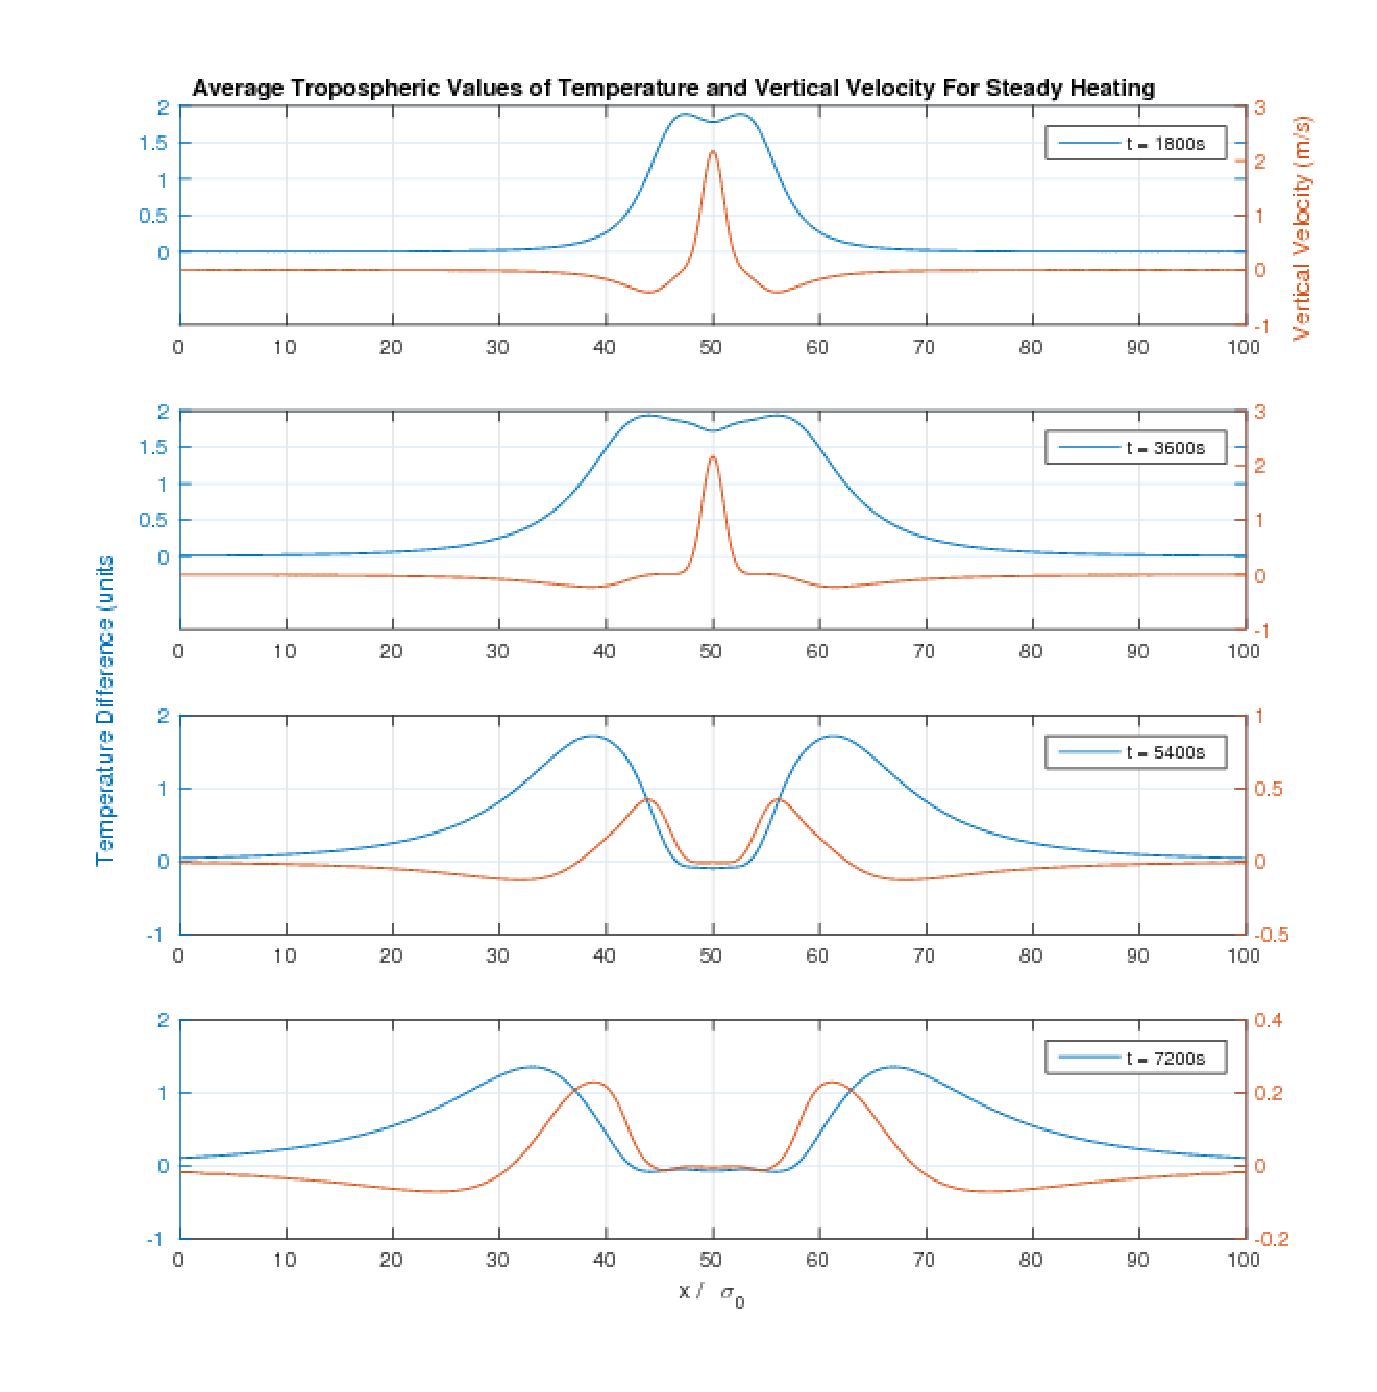
\includegraphics[width=1\textwidth]{trop_values_transient.pdf}
  \label{trop_values_transient}
\end{figure}




\end{document}
